\documentclass{classeENS}
\usepackage{lipsum}
\usepackage[backend=bibtex,style=authoryear,natbib=true]{biblatex} % Use the bibtex backend with the authoryear citation style (which resembles APA)
\addbibresource{biblio.bib} % The filename of the bibliography
\usepackage[autostyle=true]{csquotes} % Required to generate language-dependent quotes in the bibliography

\usepackage{algorithm}
\usepackage{algorithmicx}
\usepackage{algpseudocode}
\usepackage{amsmath}
\usepackage{amssymb}
\usepackage{comment}
\usepackage{mathtools, stmaryrd}
\usepackage{parskip}
\usepackage{titlesec}

\setcounter{secnumdepth}{4}
\setcounter{tocdepth}{3}
\makeatletter
\newcounter{subsubsubsection}[subsubsection]
\renewcommand\thesubsubsubsection{\thesubsubsection .\@alph\c@subsubsubsection}
\newcommand\subsubsubsection{\@startsection{subsubsubsection}{4}{\z@}%
                                     {-3.25ex\@plus -1ex \@minus -.2ex}%
                                     {1.5ex \@plus .2ex}%
                                     {\normalfont\normalsize\bfseries}}
\newcommand*\l@subsubsubsection{\@dottedtocline{3}{10.0em}{4.1em}}
\newcommand*{\subsubsubsectionmark}[1]{}
\makeatother

\usepackage{array,multirow,makecell}
\setcellgapes{1pt}
\makegapedcells
\newcolumntype{R}[1]{>{\raggedleft\arraybackslash }b{#1}}
\newcolumntype{L}[1]{>{\raggedright\arraybackslash }b{#1}}
\newcolumntype{C}[1]{>{\centering\arraybackslash }b{#1}}
\newcolumntype{M}[1]{>{\centering}m{#1}}

\setlist[itemize]{label=\textbullet}

\title{Template rapport ENS} %Titre du fichier

\begin{document}

%----------- Informations du rapport ---------

\titre{Internship report} %Titre du fichier .pdf
\departement{Computer Graphics} 
\matiere{} 
\motif{}

\enseignant{Gurprit Singh} %Nom de l'enseignant
%\tuteurpcp{}
\eleves{Pacôme \textsc{Luton}} %Nom des élèves

%----------- Initialisation -------------------
        
\fairemarges %Afficher les marges
%\fairepagedegarde
\tabledematieres %Créer la table de matières
%\tabledefigure

%------------ Corps du rapport ----------------

\section{Introduction}

\> This work is an invitation to the journey I followed during my internship. 
Let's start by introducing the context.

\> In 3D rendering, we often need to calculate integrals numerically. 
For instance when we want to compute the global illumination of a scene,
or simply when when want to find the color of a pixel by averaging all
value of illumination inside the pixel [\cite{DBLP:journals/tog/RamamoorthiAMN12}]. 

\> In the general case, this problem is difficult. Often the best we 
can do is to calculate an approximation of this integral. For this 
purpose, Monte Carlo integration is used. This method works well in 
all cases. But if we have additional information about the shape of 
the function we are integrating then we can do better. That is, we can 
find a way to calculate the integral faster and with a better approximation 
[\cite{singh17convergence}].

\> So I looked at a particular case of functions where we know the global
shape of its power spectrum. I used different methods 
to see what we could do in order improve the quality of our approximation
for those particular functions. 

%-------------------------------------------------------------------------
\section{Preliminaries}

\begin{figure}[H]
    \centering
    \begin{tabular}{C{2cm} L{10cm}}
    \hline  
        Symbol & Description
    \tabularnewline 
    \hline
        $I$ & integral of a function
    \tabularnewline
        $I_N$ & Monte Carlo estimator of I
    \tabularnewline
        $S$ & sample function
    \tabularnewline
        $\mathcal F_f$ & fourier transform of the function $f$
    \tabularnewline
        $\mathcal P_f$ & power spectrum of the function $f$
    \tabularnewline
        $Var(.)$ & the variance function
    \tabularnewline
        $W_p$ & Wasserstein distance
    \tabularnewline
        $SW_p$ & slice Wasserstein distance
    \tabularnewline
        $D_N^*$ & discrepancy
    \tabularnewline
        $B$ & a set of hihg dimensional rectangle
    \tabularnewline
        $card(.)$ & cardinality of a set
    \tabularnewline
    \hline 
    \end{tabular}
\end{figure}

\subsection{Monte Carlo}

Before going further into what I have done, here is a brief 
introduction to Monte Carlo integration. We want to compute integrals of 
the form:
    \[ I = \int_{\mathbb A} f(x) dx\]
where $\mathbb A$ is the $d$ dimensional euclidean space.

\> \textit{Monte Carlo integration}. Monte Carlo integration is an approximation
    $I_N$ of the integral $I$ by evaluation $f$ in $N$ random points $\{x_j\}_{j=1}^N$ uniformly 
    distributed over the space $A$. Formally :
    \[ I_N = \int_{\mathbb A} S(x)f(x)dx, 
        \: \text{ with } \:
    S(x) = \frac{1}{N} \sum_{j=1}^N \delta(\lVert x-x_j \rVert) \] 

\noindent We can also see this integration in the Fourier domain:
\[I_N = \int \mathcal F_S(\omega) \mathcal F_f^*(\omega) d\omega 
    \: \text{ with } \:
    \mathcal F_S(\omega) = \frac{1}{N} \sum_{j=1}^N e^{-2i\pi(\omega\cdot x_j)} \]

    \noindent where $F_f$ is the Fourier transform of $f$ and $\ F_f^*$ is the 
    complex conjugate of $F_f$.

\> \textit{Variance formulation}. Prior works [\cite{Durand2011AFA}; \cite{Pilleboue:2015:VAMCI}; \cite{10.1145/2461912.2462013}] 
    have shown that the variance of $I_N$ depends on the power spectrum of the integral 
    and the expected power spectrum of the homogenized sampling pattern:
    \[ Var(I_N) = \int_\Theta \langle \mathcal P_S(\omega)\rangle \mathcal P_f(\omega) d\omega \]
    \noindent where $\Theta = \mathbb R^d\backslash\{0\} $

%\> \textit{Radial Average Variance Formulation}. As explain in [\cite{singh17convergence}] and [\cite{Pilleboue:2015:VAMCI}],
%    we can also formulate this equation by making radial average.
%    \[ Var(I_N) = \int_0^\infty \rho^{d-1} \int_{\mathbb{S}^{d-1}} \langle \mathcal P_S(\rho \textbf{n})\rangle \mathcal P_f(\rho \textbf{n}) d\textbf{n} d\rho\]
%    Or, if we inverse the integral, we get:
%    \[ 
%        Var(I_N) = \int_{\mathbb{S}^{d-1}} \int_0^\infty \rho^{d-1} \langle \mathcal P_S(\rho \textbf{n})\rangle \mathcal P_f(\rho \textbf{n}) d\rho d\textbf{n} \]
    
%    {\color{red} TO REMORFULATE, BUT THIS IS THE MAIN IDEA THAT EXPLAIN THE LIMITATION OF WHAT I AM DOING, SO IT IS REALLY IMPORTANT}\\
%\> \textit{Remark on Sample Power Spectrum} Intuitively, if we want to distribute well N
%    samples in a hypercube of volume $1$. Each sample will cover in average a volume of
%    $1/N$. Since there is a strong link between PCF and power Spectrum. The volume of
%    low value close to zero in the power spectrum could in the best case be $O(N)$.\\
%    {\color{red} The idea behind is that, if we want to optimize for a constant subset of
%    $\mathbb{S}^{d-1}$ that is not negligible, we can at most achieve a dark region of 
%    size $O(1/N^{1/d})$ in all direction}
    
\subsection{Spectral analyse of some function}

\> This formulation of the variance with power spectrum tells us 
    that if we want to reduce the variance, we need to match the 
    spectrum of our point distribution with that of the function 
    we are integrating.

\> For instance, in the paper [\cite{singh17convergence}], they showed that for 
    some rendering function, we may have some improvement in the 
    convergence rate of our approximation by using anisotropic 
    sample distribution.

\> During this internship, I focused on one particular form of function.
    Lets $f\in\mathcal C(\mathbb R^d,\mathbb R)$ be a function that 
    is aligned along a vector $v \in \mathbb R^d$. That means that:
    \[ \forall x\in\mathbb R^d, \forall \lambda\in\mathbb R f(x+\lambda v) = f(x) \]
    We can then compute the Fourier transform of this function:
    \begin{align*}
        f(\xi) &= \int_{\mathbb R^d} f(x) e^{-2i\pi \xi\cdot x} dx \\
               &= \int_{y\cdot v=0, \lambda \in \mathbb R } f(y+\lambda v) 
                                    e^{-2i\pi \xi\cdot (y+\lambda v)} dy d\lambda
    \end{align*}
    With this formulation, if $\xi \cdot v \neq 0$ mod $2\pi$, we can do the integral separation : \begin{align*}
        f(\xi) &= \int_{-\infty}^{+\infty} e^{-2i\pi 
            \xi\cdot\lambda v} \int_{y\cdot v=0} f(y) e^{-2i\pi \xi\cdot y}  dy d\lambda \\
            &= \int_{-\infty}^{+\infty} e^{-2i\pi 
            \xi\cdot\lambda v} C^{te} d\lambda \\
            &= 0
    \end{align*}
    What this means is that the power spectrum of such function will be non-zero only on
    the orthogonal hyperplan to $v$ (With some copy further in the space). We note it: 
    $\mathbb R^d_{\perp v} = \{x \in \mathbb R^d | x.v = 0\}$.

\> And, by the linearity of the Fourier transform, if our function $f = \sum_i f_i$ is a finite sum 
    of function, where $f_i$ is aligned with $v_i$. Then, the power spectrum 
    of our function $f$ will be non-zero in the subspace 
    $A = \bigcup \mathbb R^d_{\perp v_i}$.

\> In rendering, we can encounter this type of function. For instance, 
    we typically have a function that has this property with motion blur [\cite{singh17convergence}], 
    or simply light occultor [\cite{journals/tog/EganHDR11}].
    Here is an example of a function that we might want to integrate, with her power
    spectrum, and the corresponding power spectrum of sample we want.


    \begin{figure}[H]
        \centering
        \begin{tabular}{ccc}
        \frame{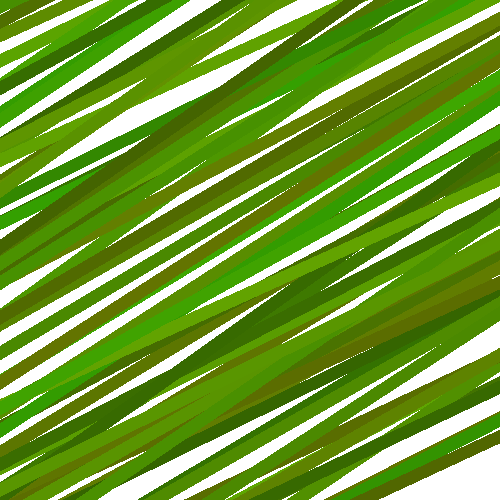
\includegraphics[width=48mm]{target/2D_fun.png}}
        &\frame{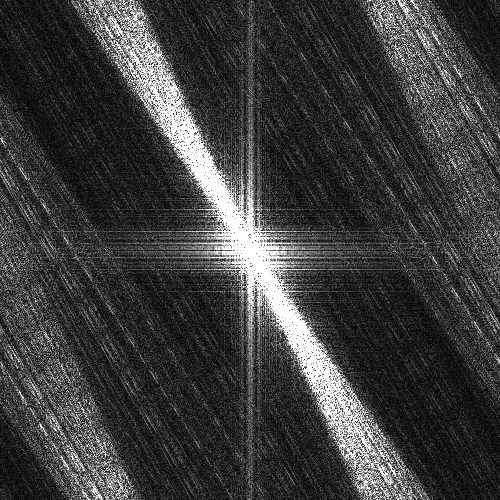
\includegraphics[width=48mm]{target/2D_spectrum.png}}
        &\frame{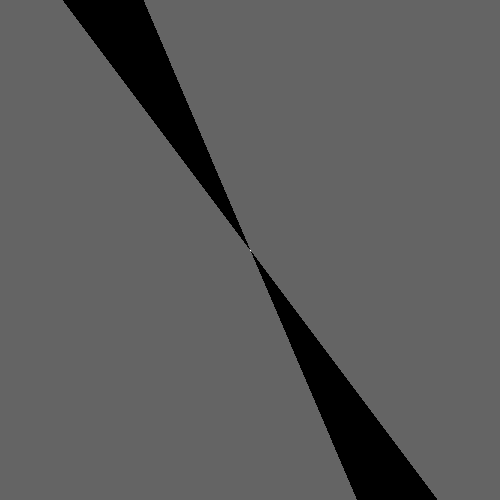
\includegraphics[width=48mm]{target/2D_target.png}}
        \\[3pt]
        $(a)$ & $(b)$ & $(c)$
        \end{tabular}
        \textit{Where $(a)$ is the function we want to integrate, $(b)$ is the power
        spectrum of this function. And $(c)$ is the power spectrum we want to target 
        for our sample.}
    \end{figure}
    
\> \textit{Remark.} An other type of anisotropic function we're interested in, 
    is the one that are close to be axes aligned. So the power spectrum 
    targeted is a cross aligned with the axis [\cite{singh17convergence}]. 
    This is one of the reason why 
    low discrepancy sampler are so effective.

\section{Anisotropic sample}

During this work, I used four different ways of creating sample distribution:
\begin{itemize}
    \item Radial Average Target
    \item Relaxation method
    \item Optimal Transport with Wasserstein
    \item Slice Optimal Transport 
\end{itemize}
All the proofs and the description of those methods are in Annexe. 
You don't have to read how they work to understand the rest of this work.

\subsection{Radial Average algorithm}
    The first method I tried is to optimize directly for a target power spectrum.
    This method only requires to have a radial average target distribution. Thus, we can
    target a Blue Noise distribution, but we can also target a step noise distribution.
    
    We can also change a bit the algorithm, and instead of taking the all radial average,
    we can take only a part of the angle. For instance, we could take the average for
    point in the power spectrum that are in $[\frac{4\pi}{3} - 0.1, \frac{4\pi}{3}+0.1]$
    
\begin{figure}[H]
        \centering
        \begin{tabular}{ccc}
        \frame{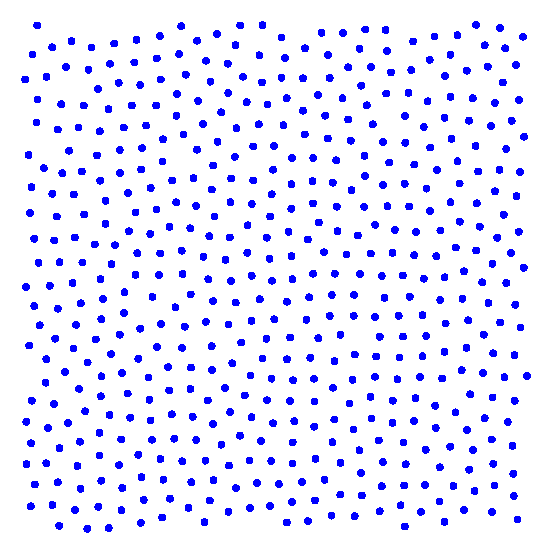
\includegraphics[width=48mm]{sample/SGD_blue.pdf}}
        &\frame{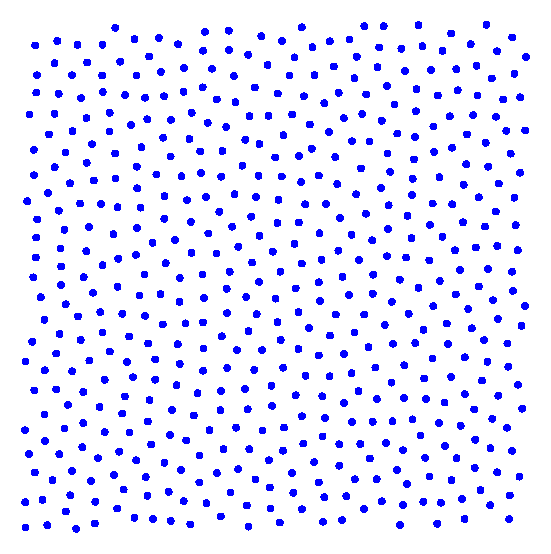
\includegraphics[width=48mm]{sample/SGD_step.pdf}}
        &\frame{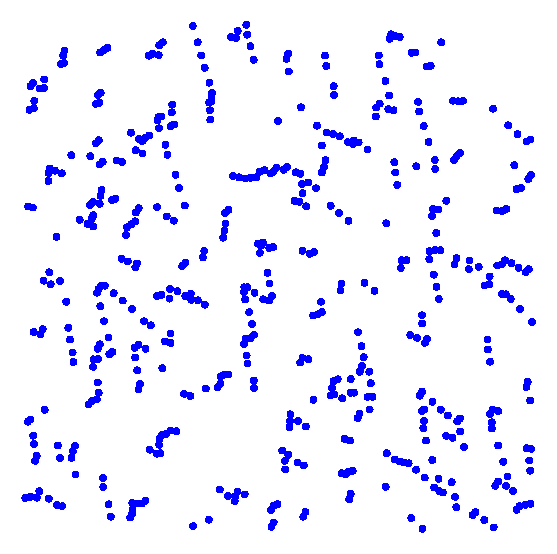
\includegraphics[width=48mm]{sample/SGD_dw.pdf}}
        \\[3pt]
        \frame{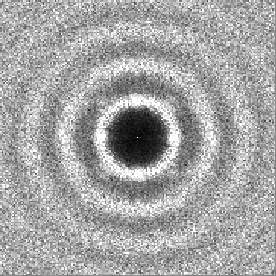
\includegraphics[width=48mm]{sample/SGD_blue.png}}
        &\frame{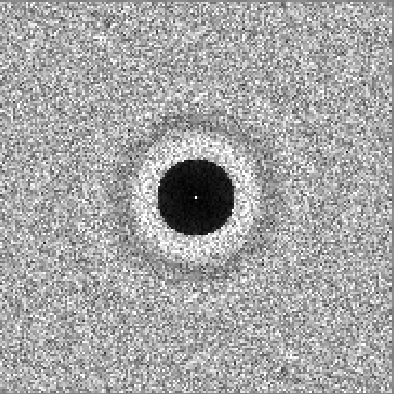
\includegraphics[width=48mm]{sample/SGD_step_spectrum.png}}
        &\frame{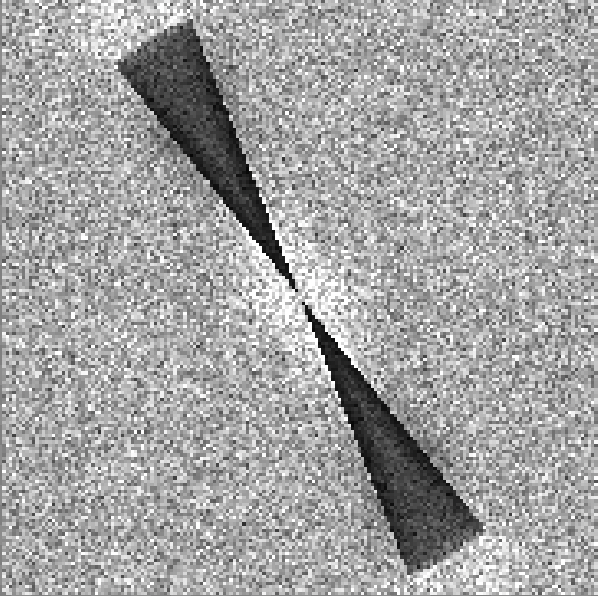
\includegraphics[width=48mm]{sample/SGD_dw_spectrum.png}}
        \\[3pt]
        \frame{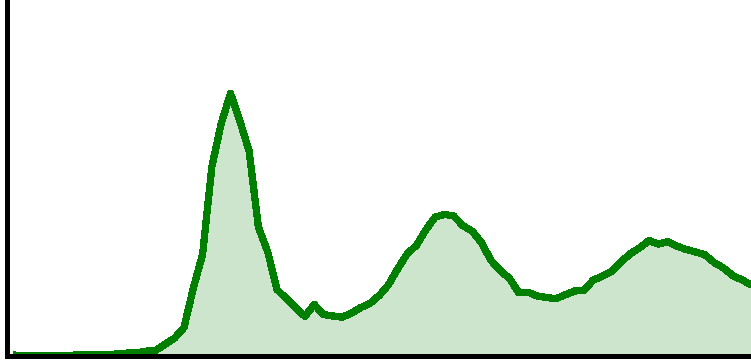
\includegraphics[width=48mm]{sample/SGD_blue_radial.pdf}}
        &\frame{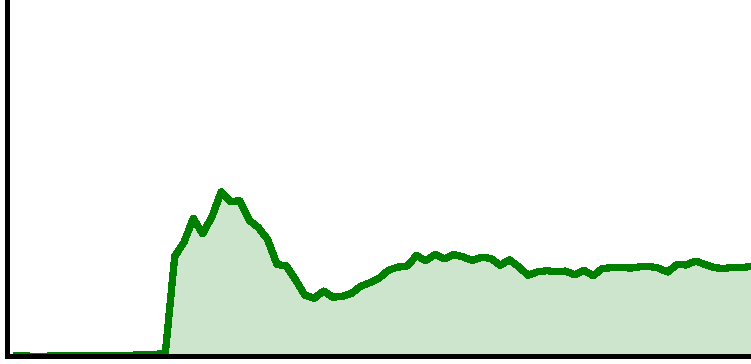
\includegraphics[width=48mm]{sample/SGD_step_radial.pdf}}
        &\frame{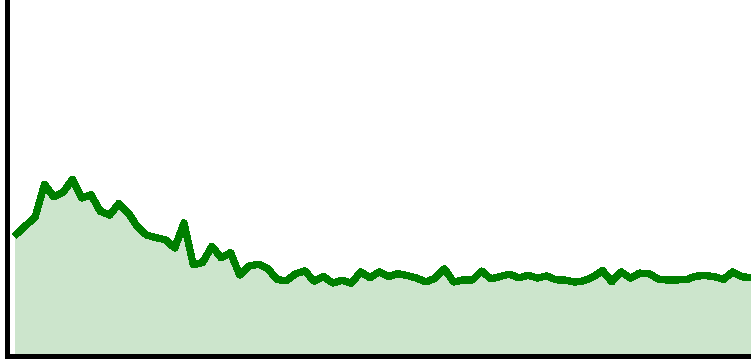
\includegraphics[width=48mm]{sample/SGD_dw_radial.pdf}}
        \\[3pt]
        \textit{Blue noise} & \textit{Step noise} & \textit{Double wedge}
        \end{tabular}
    \end{figure}
    
\> \textit{Discussion}. The method has the advantage of being explicit. The blue noise
    generated isn't of highest quality. The sample for the double wedge 
    spectrum look terrible. But the main issue with this method, is that it doesn't scale
    well. The time needed to generate a sample increase more than quadratically. 

%\> \textit{For fun}. In fact, maybe we could be able to draw any drawing in the power
%    spectrum. {\color{red} TO DO : try to do a nice drawing}

\subsection{Modified SOT}

\> A PhD from the lab, Corentin Salaün, discovered that with Slice Optimal Transport, 
if instead of optimizing for the classical SOT (more detail about how  it works can be found in the annexe):
\[SW_p(\mu, \nu) = \int_{\mathbb{S}^{d-1}} W_p(\mu^\theta,\nu^\theta) d\theta\]
We optimise for:
\[SW_p(\mu, \nu) = \int_{\mathbb{S}^{d-1}} \gamma(\theta) W_p(\mu^\theta,\nu^\theta) d\theta\]
where $\gamma$ is a probabilistic measures on $\mathbb{S}^{d-1}$. Then we can get anisotropic
power spectrum. And even better, the impact on the power spectrum seems to depend linearly to
the probabilistic measures we used.

\> \textit{Discussion}. The idea behind, is that by doing so, we will privileged some
    direction on other. And thus, we hope the by doing so, our sample we be better in
    those direction than if we had optimize every direction.
    
\> \textit{Remark}. The Slice Optimal Transport blue noise is obtain when 
    $\gamma$ is uniformly distributed over $\mathbb{S}^{d-1}$.

\subsubsection{Double wedge spectrum}

\subsubsubsection{Simple double wedge}
\textit{Objective} Like introduce in section $2.2$, we want to create sample distribution
    that have a power spectrum that is a double wedge. In order to do so, we can take
    a well chosen $\gamma$ like describe below:

In the 2D euclidean domain. $\mathbb{S}^{d-1}$ is isomorphe to angle $\theta \in [0,2\pi]$.
So if instead of taking $\gamma$ uniform distribution on $[0,2\pi]$, we take $\gamma$
uniform distribution on $[\theta_0,\theta_1]$ we get this sample.

\begin{figure}[H]
    \centering
    \begin{tabular}{cccc}
    \frame{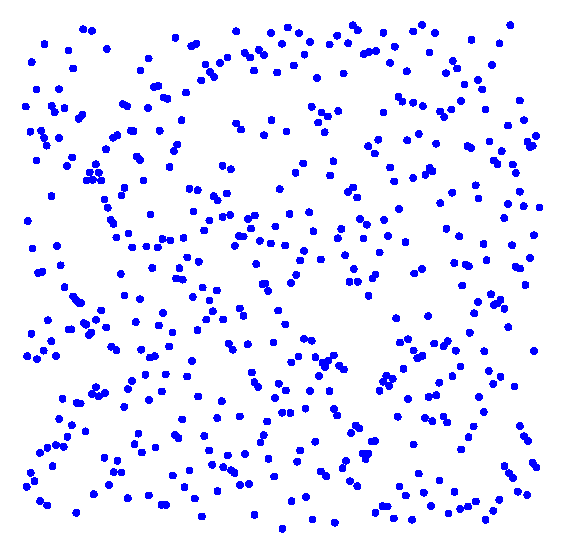
\includegraphics[width=33mm]{sample/dw1.pdf}}
    & \frame{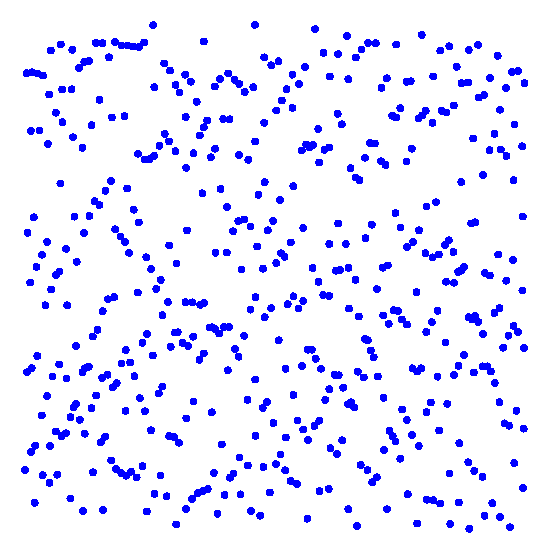
\includegraphics[width=33mm]{sample/dw2.pdf}}
    & \frame{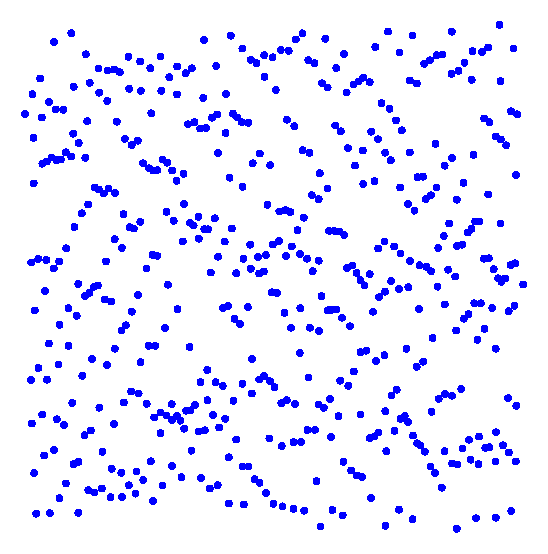
\includegraphics[width=33mm]{sample/dw3.pdf}}
    & \frame{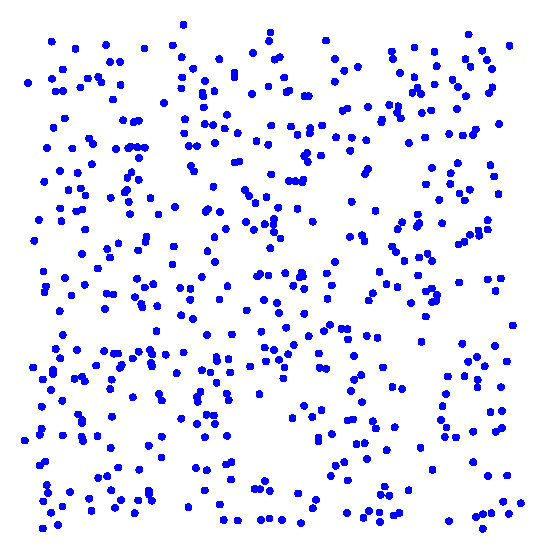
\includegraphics[width=33mm]{sample/dw1b.pdf}}
    \\[3pt]
    \frame{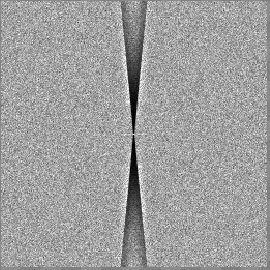
\includegraphics[width=33mm]{sample/dw_1.png}}
    & \frame{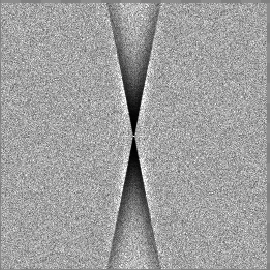
\includegraphics[width=33mm]{sample/dw_2.png}}
    & \frame{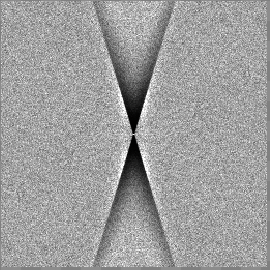
\includegraphics[width=33mm]{sample/dw_3.png}}
    & \frame{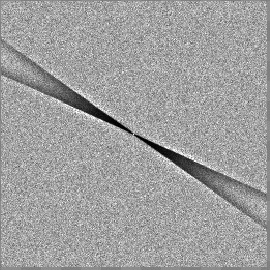
\includegraphics[width=33mm]{sample/dw_1b.png}}
    \\[3pt]
    \textit{(dw1)} & \textit{(dw2)} & \textit{(dw2)} & \textit{(dw1b)}
    \end{tabular}\\
    \textit{Where, (dw1) correspond to $\theta \in [-0.1,0.1]$, 
                   (dw2) correspond to $\theta \in [-0.2,0.2]$,\\
                   (dw3) correspond to $\theta \in [-0.3,0.3]$ and
                   (dw1b) correspond to $\theta \in [-0.1, +0.1] +\frac{\pi}{3}$}
\end{figure}

Theoretical, in the ideal world this should improve the convergence for function aligned 
in some direction. But in practice, because we don't integrate on infinite domain, all
function have at least small but none zero low frequency value in almost all direction. 

A really good way of seeing the trade off of this sample is to integrate a rectangle
function in every direction, and plot the variance according to the direction of 
rectangle function.

    \begin{figure}[H]
        \centering
        \begin{tabular}{cc}
            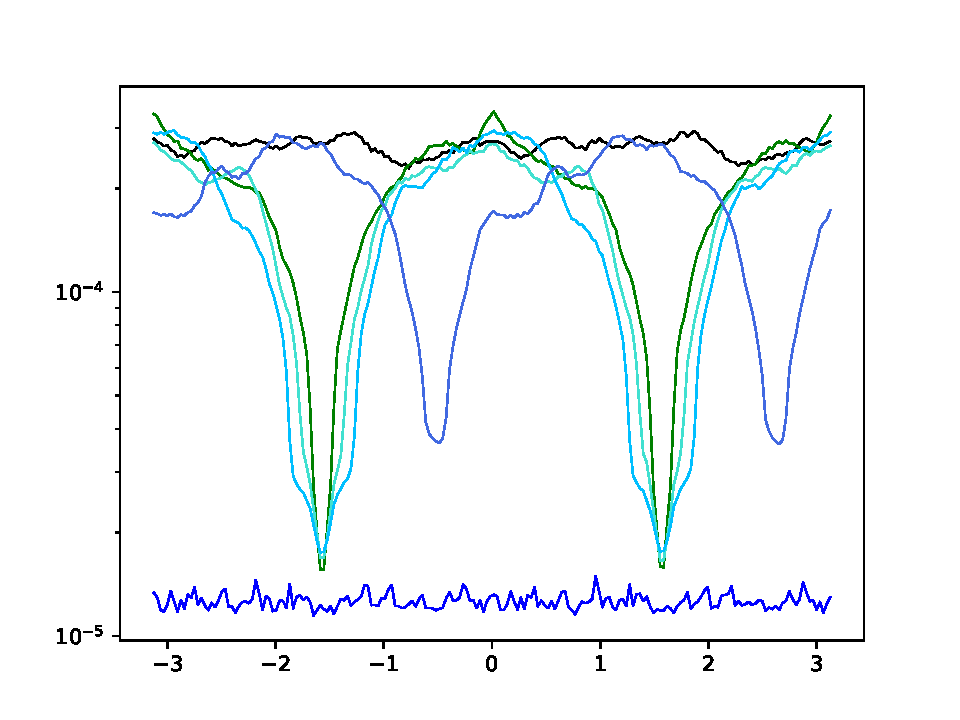
\includegraphics[width=120mm]{plot/integration_rot_bad.pdf}
            & \frame{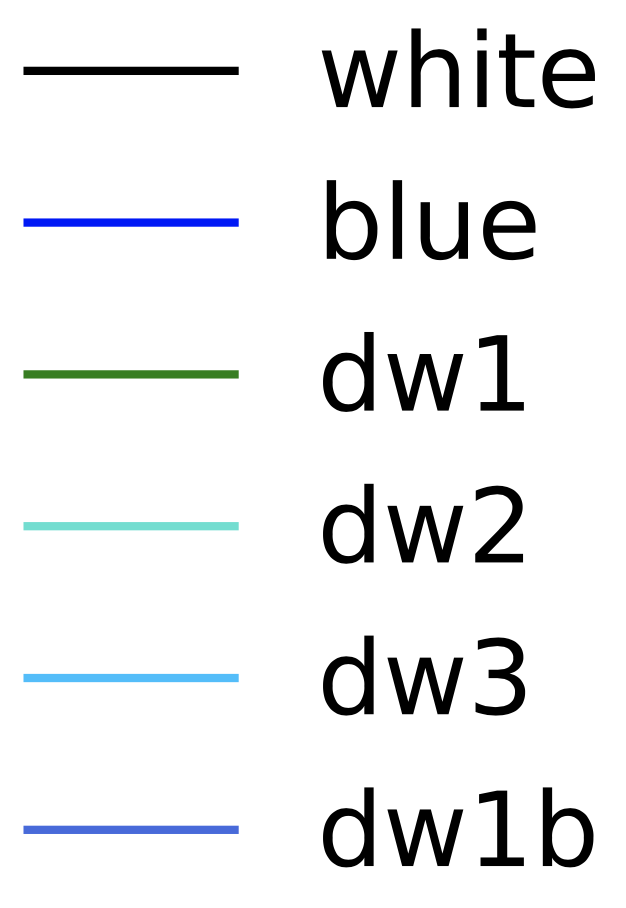
\includegraphics[width=20mm]{plot/legend.png}}
        \end{tabular}\\
        \textit{The X-axis is the angle of orientation of the rectangle, and the Y-axis
        correspond to the means square error. The rectangle we integrate is $0.96$ unit long and $0.12$ unit width}\\
        
    \end{figure}    


\> \textit{Remark}. We use a rectangle instead of a Heaviside function in order to have
    a shape that is consistent when we rotate it. The size of the frontier of an 
    Heaviside function change with the orientation, thus, it will produce some artefact.


As the figure show, with this we don't even beat in one direction simple slice optimal
    transport blue noise. 
    
\subsubsubsection{Better double wedge}

    In order to face this issue, one solution is to do a mixture 
    of $\gamma$. It is the same idea than multi importance sampling.
 \[ \gamma = (1-p) \gamma_{uniform} + p\gamma_{double wedge} \]
Here, we set $p = 0.8$
\begin{figure}[H]
    \centering
    \begin{tabular}{cccc}
    \frame{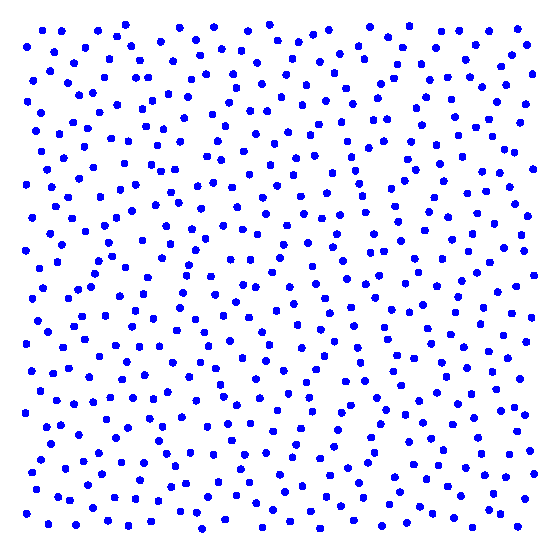
\includegraphics[width=33mm]{sample/dwb1.pdf}}
    & \frame{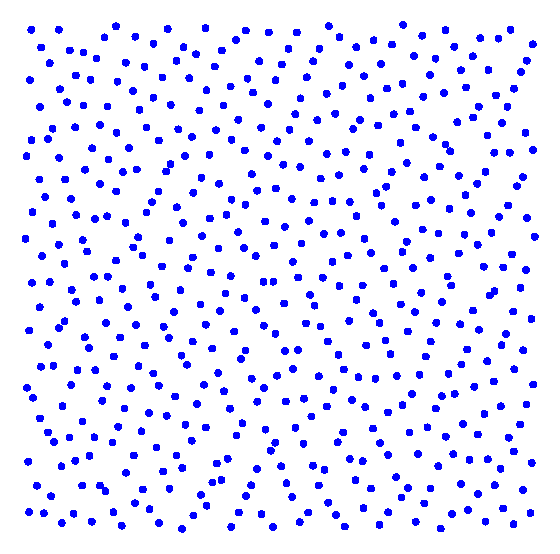
\includegraphics[width=33mm]{sample/dwb2.pdf}}
    & \frame{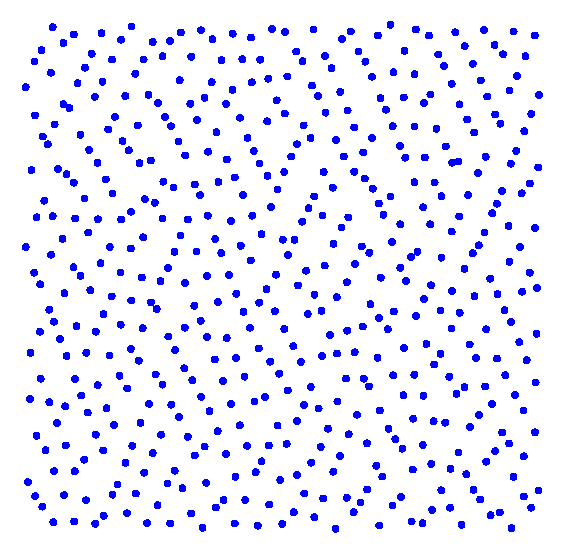
\includegraphics[width=33mm]{sample/dwb3.pdf}}
    & \frame{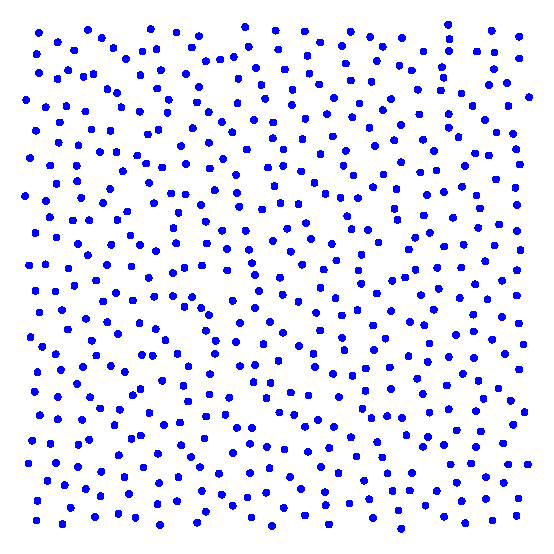
\includegraphics[width=33mm]{sample/dwb1b.pdf}}
    \\[3pt]
    \frame{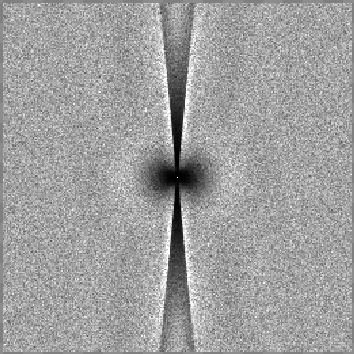
\includegraphics[width=33mm]{sample/dwb1.png}}
    & \frame{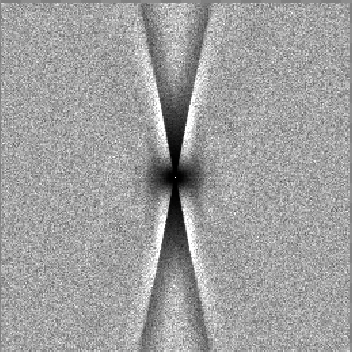
\includegraphics[width=33mm]{sample/dwb2.png}}
    & \frame{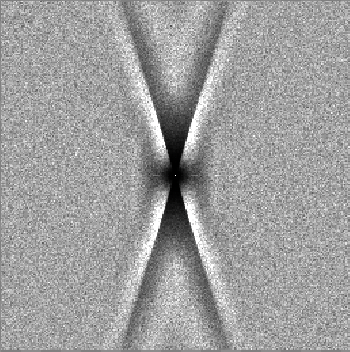
\includegraphics[width=33mm]{sample/dwb3.png}}
    & \frame{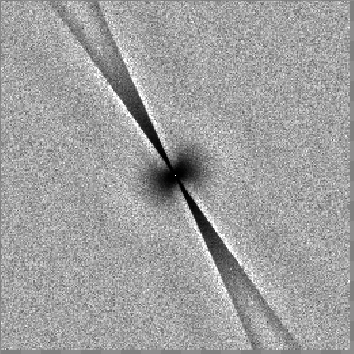
\includegraphics[width=33mm]{sample/dwb1b.png}}
    \\[3pt]
        \textit{(dw1)} & \textit{(dw2)} & \textit{(dw2)} & \textit{(dw1b)}
    \end{tabular}\\
    \textit{Where, (dw1) correspond to $\theta \in [-0.1,0.1]$, 
                   (dw2) correspond to $\theta \in [-0.2,0.2]$,\\
                   (dw3) correspond to $\theta \in [-0.3,0.3]$ and
                   (dw1b) correspond to $\theta \in [-0.1, +0.1] +\frac{\pi}{3}$}
\end{figure}

With this change, we can compute the same plot that previously and we get:
    
    \begin{figure}[H]
        \centering
        \begin{tabular}{cc}
            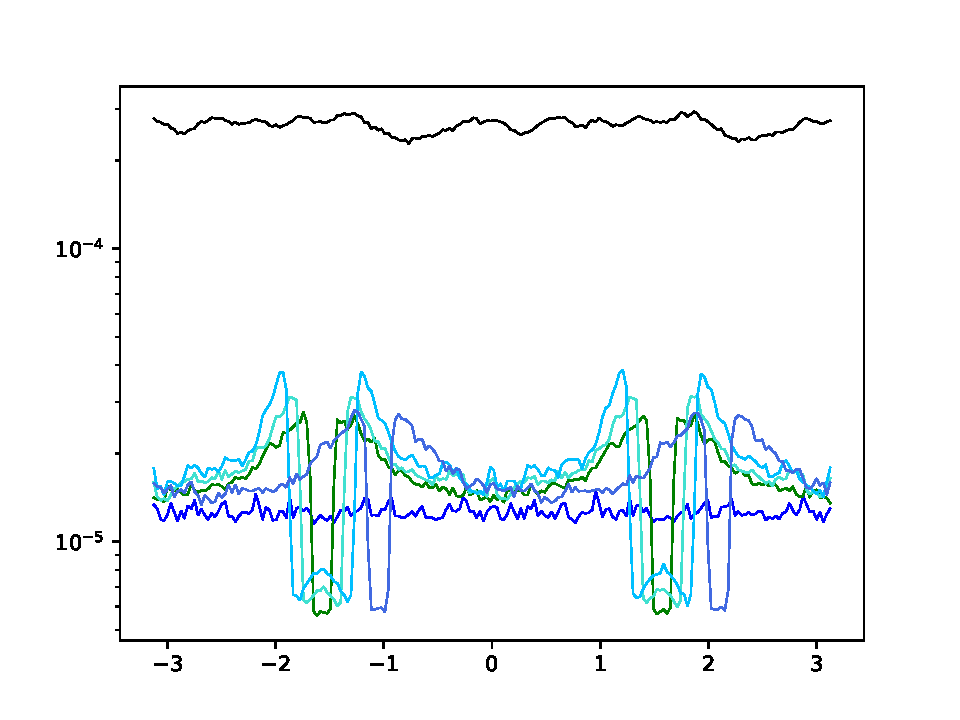
\includegraphics[width=120mm]{plot/integration_rot_good.pdf}
            & \frame{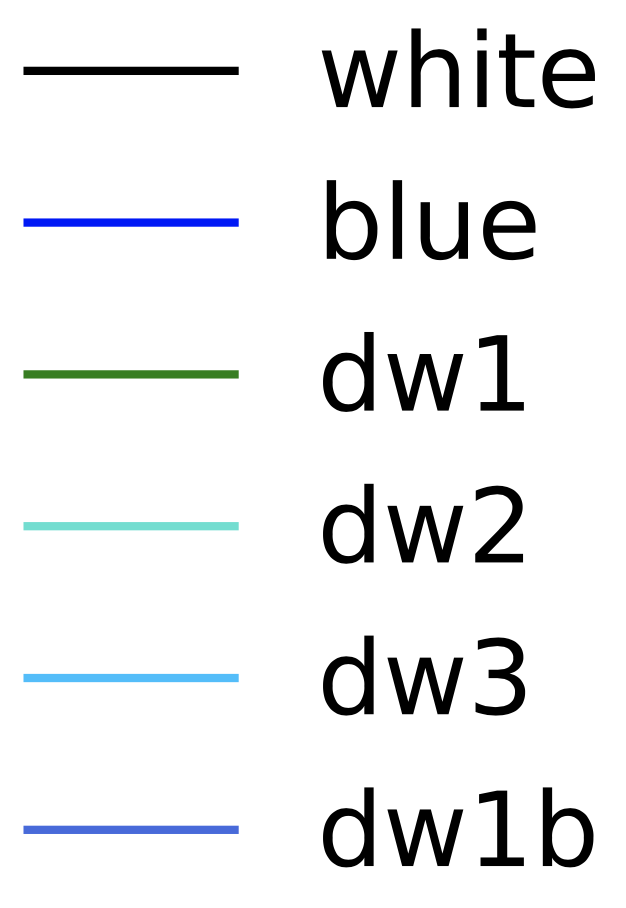
\includegraphics[width=20mm]{plot/legend.png}}
        \end{tabular}
    \end{figure}  

Now we can clearly see improvement for some direction. To better see those improvement in
some particular direction, here are plot of means square error when $N$ increase:

    \begin{figure}[H]
        \centering
        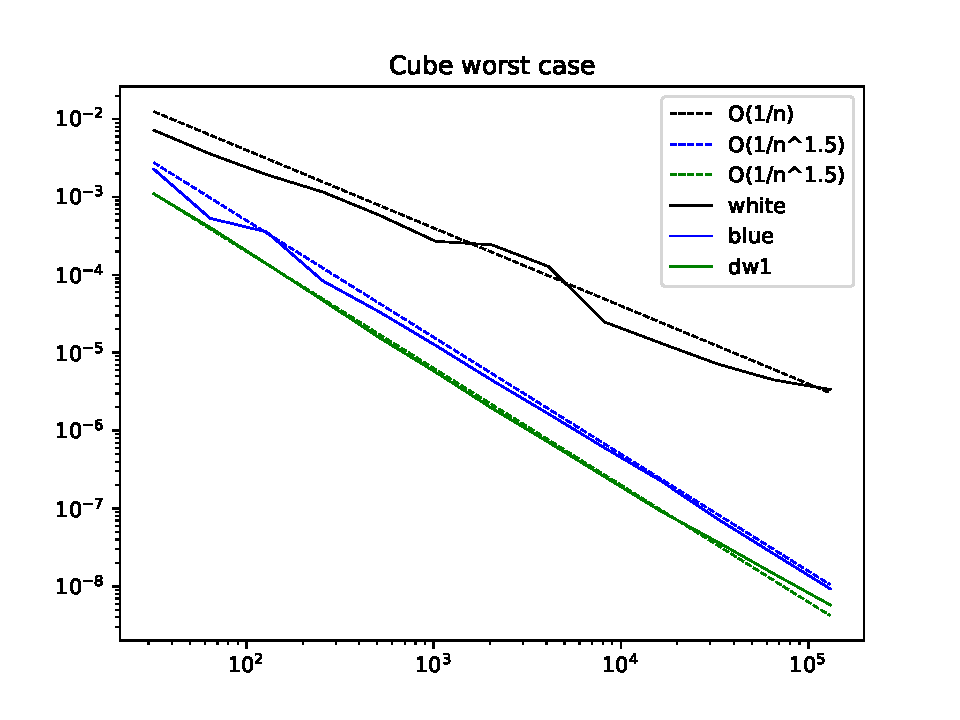
\includegraphics[width=110mm]{plot/integration_rec_dw.pdf}\\
    \end{figure}  

\>  But, in reality, as the previous plot show, those improvement, are 
    only a constant time better than 
    blue noise. In order to have achieve a new order of convergence, we would need to
    make the size of the interval depends on the number of sample. Intuitively, the power 
    spectrum of a sample is like having $O(N)$ quantity of dark region, due to his strong 
    link with PCF (pair correlation function).

\subsubsection{Cross in 2D}

\textit{Objective} Like introduce in section $2.2$, we also want to create sample
    distribution that have a power spectrum that is cross. In order to do so, we 
    can take a well chosen $\gamma$ like describe below:

\subsubsubsection{How to make a cross}

If we choose $\gamma$ to be the distribution of a cross, then if we sample $\gamma$ to 
compute our SOT (this is some importance sampling), we will get a cross. To do so, we need 
to inverse the probabilistic measures.

Let $l$ be the ratio between to length and wide of the cross.
First we can sample $\theta \in [0,\pi/4]$. To do so, we first sample uniformly $v \in [0,(l-0.5)N]$.
And then:  
\begin{itemize}
    \item if $v < lN/2$, then  $\theta = \tan^{-1}\left (\frac{2v}{l^2N} \right )$
    \item if $v > lN/2$, than $\theta = \tan^{-1}\left (\frac{(N)}{2(lN-v)} \right )$
\end{itemize}
To make the full cross, we can then just sample which of the 8 cadran we want $\theta$ to be in.
And make the proper transformation.

\> \textit{Remark}. It is quite fast. Only two random uniform number request. It's in $O(1)$.

\subsubsubsection{Fixed size cross}

If we chose $l$ to be constant. We can get the following cross.
\begin{figure}[H]
    \centering
    \begin{tabular}{cccc}
    \frame{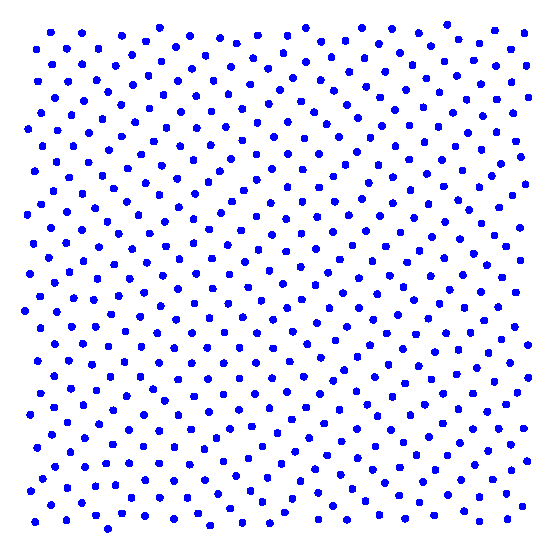
\includegraphics[width=33mm]{sample/cross2.pdf}}
    & \frame{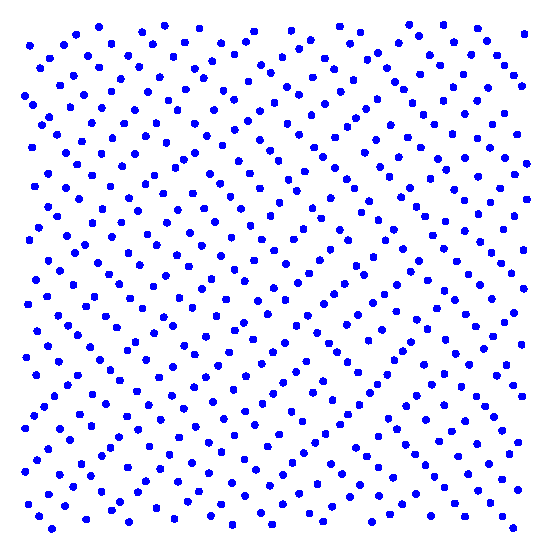
\includegraphics[width=33mm]{sample/cross5.pdf}}
    & \frame{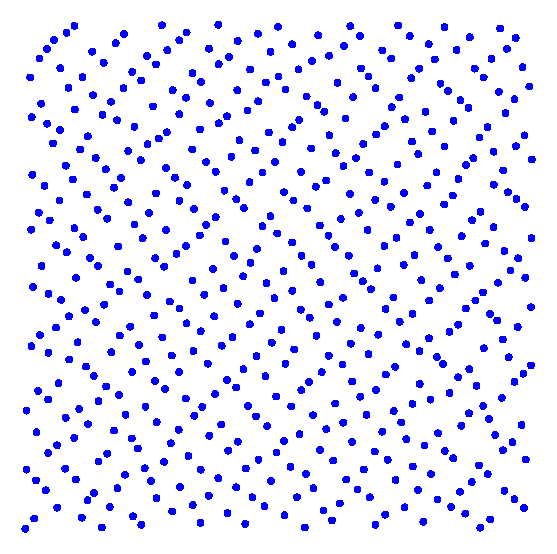
\includegraphics[width=33mm]{sample/cross10.pdf}}
    & \frame{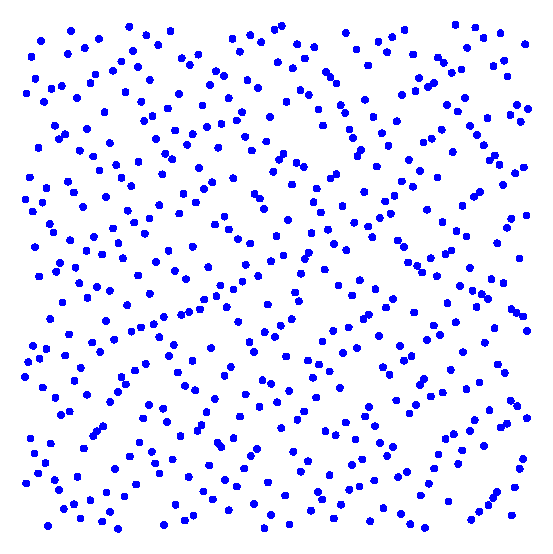
\includegraphics[width=33mm]{sample/cross40.pdf}}
    \\[3pt]
    \frame{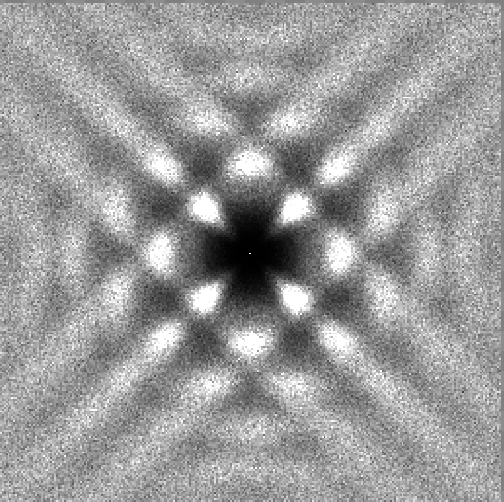
\includegraphics[width=33mm]{sample/cross2.png}}
    & \frame{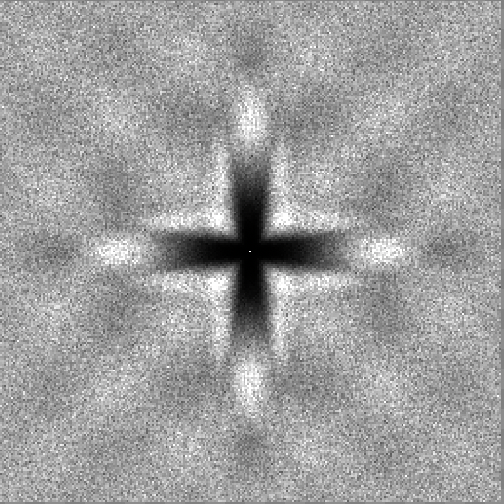
\includegraphics[width=33mm]{sample/cross5.png}}
    & \frame{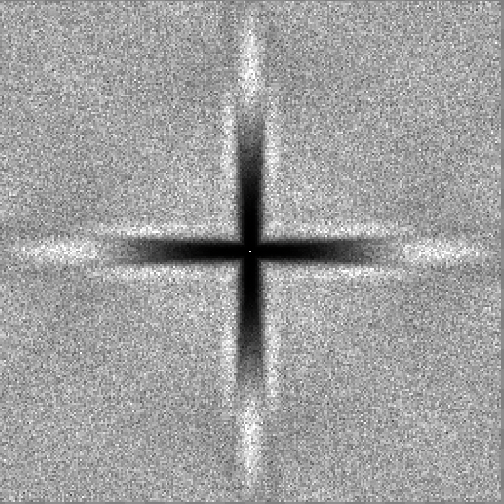
\includegraphics[width=33mm]{sample/cross10.png}}
    & \frame{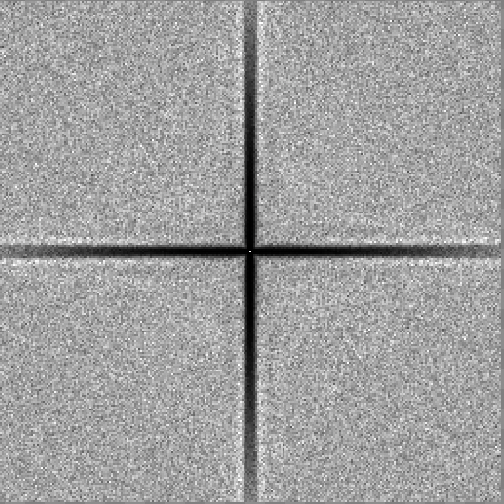
\includegraphics[width=33mm]{sample/cross40.png}}

    \\[3pt]
    $ l = 2$
    & $l = 5$ 
    & $l = 10$ 
    & $l = 40$ 
    \end{tabular}
\end{figure}
We have the same issue than with double wedge. In the worst case (integration of a 
 function align with axis), we have a lower convergence rate then Owen. And in the
 best case we only beat Owen by a constant.

\begin{figure}[H]
    \centering
    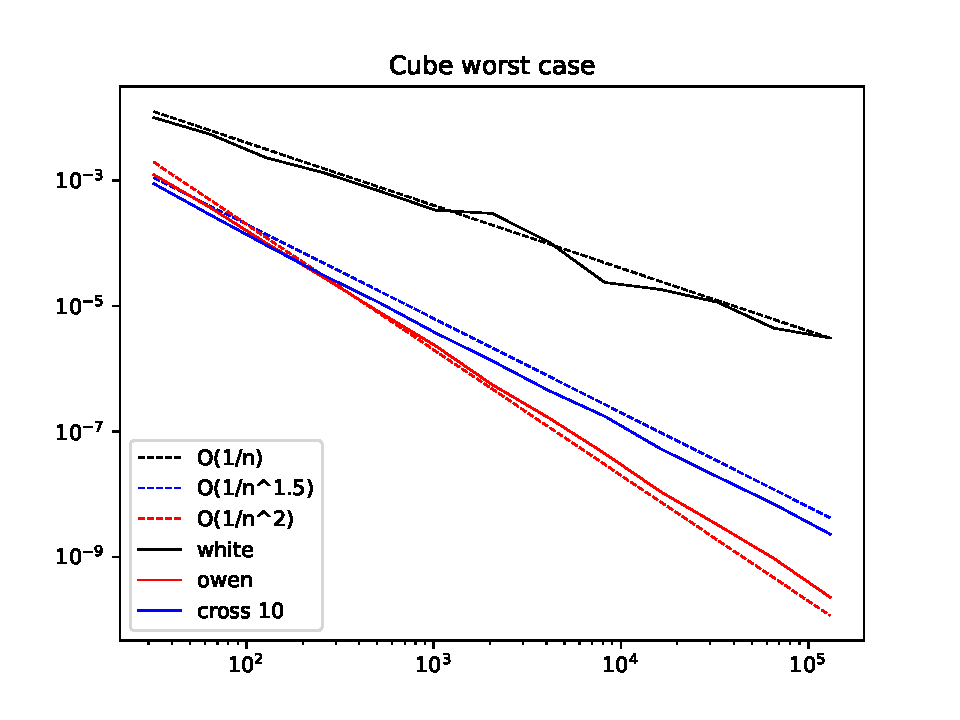
\includegraphics[width=75mm]{plot/integration_cube_worst.pdf}
    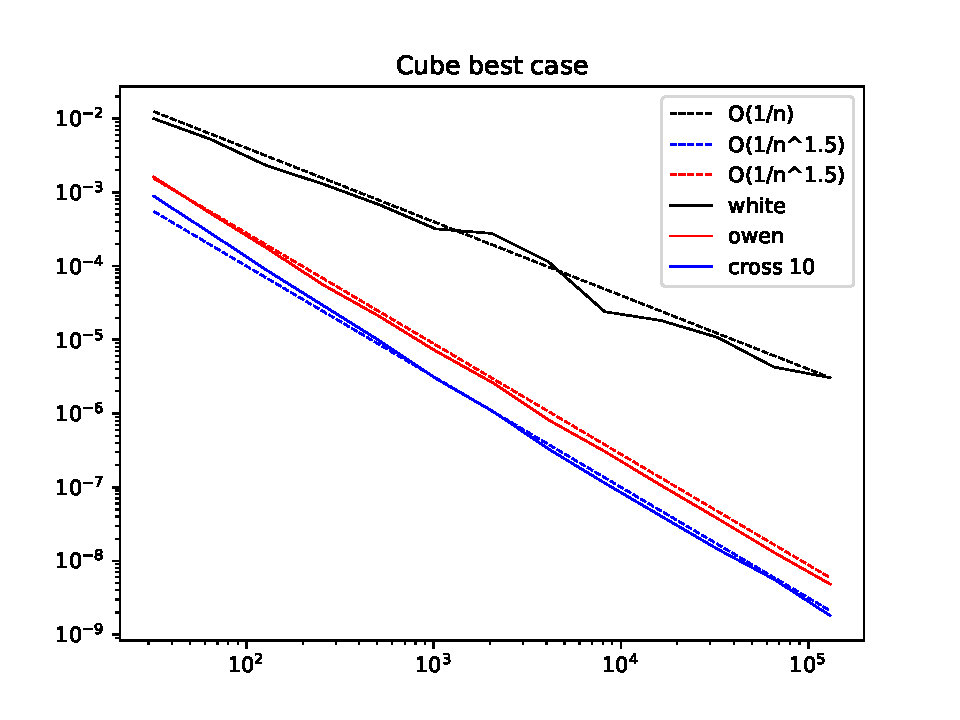
\includegraphics[width=75mm]{plot/integration_cube_best.pdf}
\end{figure}    

But, we have a better constant in front for some direction non align with the axis. Here the
integration of a cube with 1024 sample with different angle.

\begin{figure}[H]
    \centering
    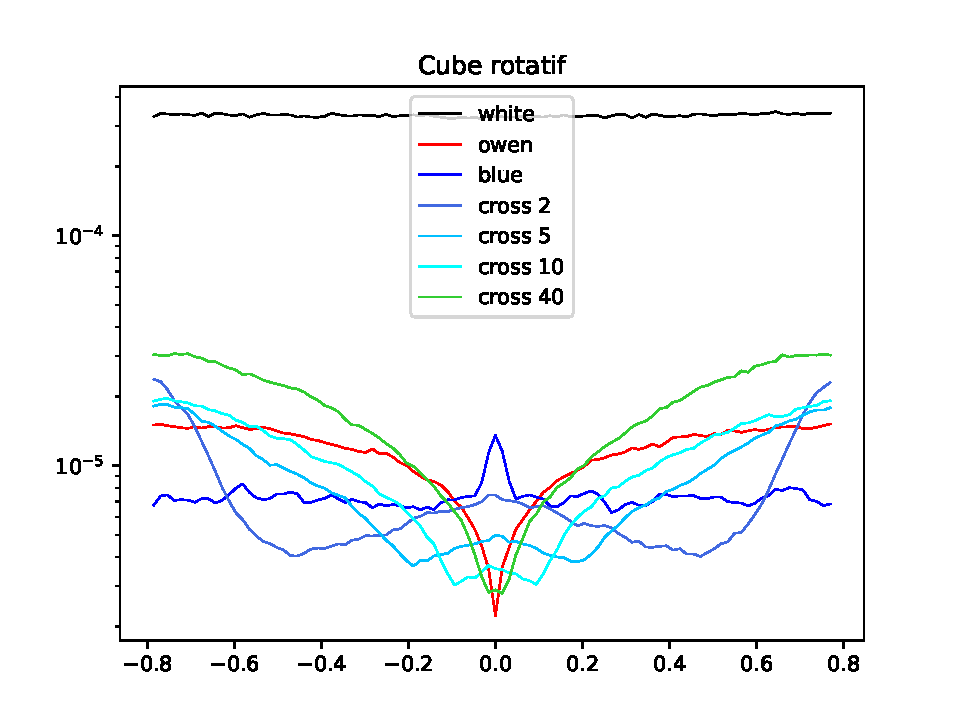
\includegraphics[width=100mm]{plot/integration_cube_rot.pdf}\\
\end{figure}    

\> \textit{Remark}. With this vision, it seems that the cross noise is a continuous morphism
    between blue noise and low discrepancy sampler like Owen.

\subsubsubsection{Moving size cross}

If we choose $l = N^{1/3}$. Then, in theory, we should have for low angle, a 
convergence rate of $O(1/N^{5/3})$ at first, followed by a convergence rate of
$O(1/N^{4/3})$.

\begin{figure}[H]
    \centering
    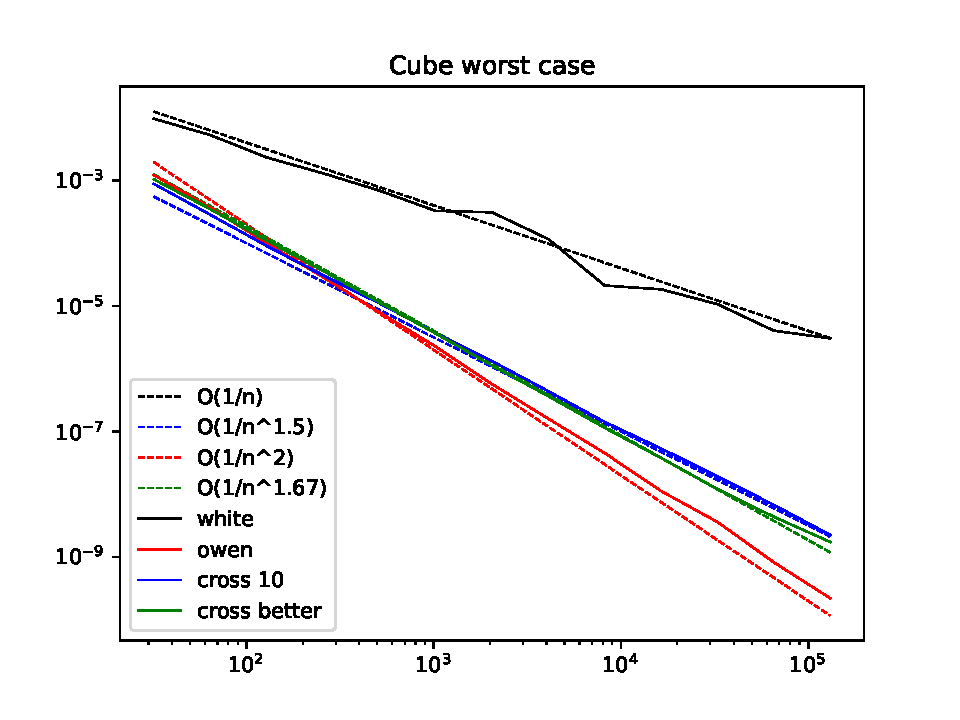
\includegraphics[width=75mm]{plot/integration_cube2_best.pdf}
    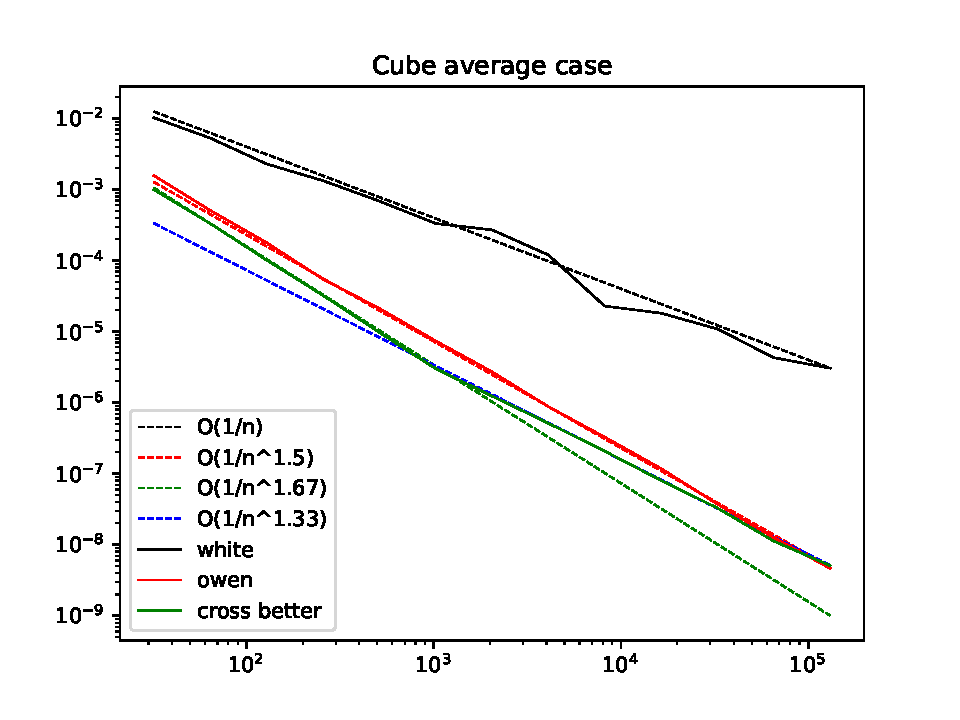
\includegraphics[width=75mm]{plot/integration_cube2_average.pdf}
\end{figure}    

\subsubsection{Discussion}

    The strength of our method, is that it is really malleable. We can do any mixture
    of shape, in order to have the best possible power spectrum. 
    
\> \textit{Fun fact.} In our last example with a cross, we can even add a third 
    convergence rate. If half of the time, we optimize for a blue noise. Formally, we use
    \[ \gamma =\frac{1}{2}\gamma_{cross} + \frac{1}{2}\gamma_{uniform}\]
    The convergence rate will follow: 
    \[ O(1/N^{5/3}) \to O(1/N^{4/3}) \to O(1/N^{3/2}) \]
    If we do a mixture of different size of cross with different coefficient, we could in theory
    make a a convergence rate that pass by any $O(N^r)$ on finite interval.

\> \textit{Why does it matter ?} More generally, theoretically, if we compute the 
    isovalue of the power spectrum of the function, and we generate sample that has 
    the same isovalue. We could improve the overall convergence rate. For example 
    if in 2D, we have a function $f$, for which the power spectrum isovalue is 
    a rectangle that decrease faster in Y-axis that in X-axis. Then we could improve the overall 
    convergence rate, by making a sample where the dark region of the power spectrum 
    follow this pattern.

\subsubsection{Attempt to 3D generalization}
    A naive way to generalized this in 3D, it to optimize along 2D projection. For instance,
    in the case of motion blur (XYT coordinate), we would like [\cite{singh17convergence}]
    \begin{itemize}
        \item the XY projection is a blue noise
        \item the XT projection is a double wedge
        \item the YT projection is a double wedge
    \end{itemize}
    But, we reality, those 2D projection don't fully describe the shape of the real 
    3D power spectrum. Thus, like n-rooks doesn't improve convergence rate in most 
    of the case, this generalization to 3D is more likely to don't improve anything
    either.
    
\> In order to improve this, I explored the impact of multiclass sampling.
    

\subsection{MultiClass sampling}

MultiClass sampling is something known in computer graphics, it can be used in
object placement [\cite{10.1145/1778765.1778816}] or for artistic stipling 
[\cite{10.1145/3478513.3480534}].

\subsubsection{Introduction to the idea}
    One things that characterize low discrepancy sampler, is that if we take the points
    within a subspace, it still has good property. For instance, if take a sub space of the
    2D euclidean space. Points inside will still have a great distribution. Just like Dyadic 
    Nets. 
    
    \begin{figure}[H]
        \centering
        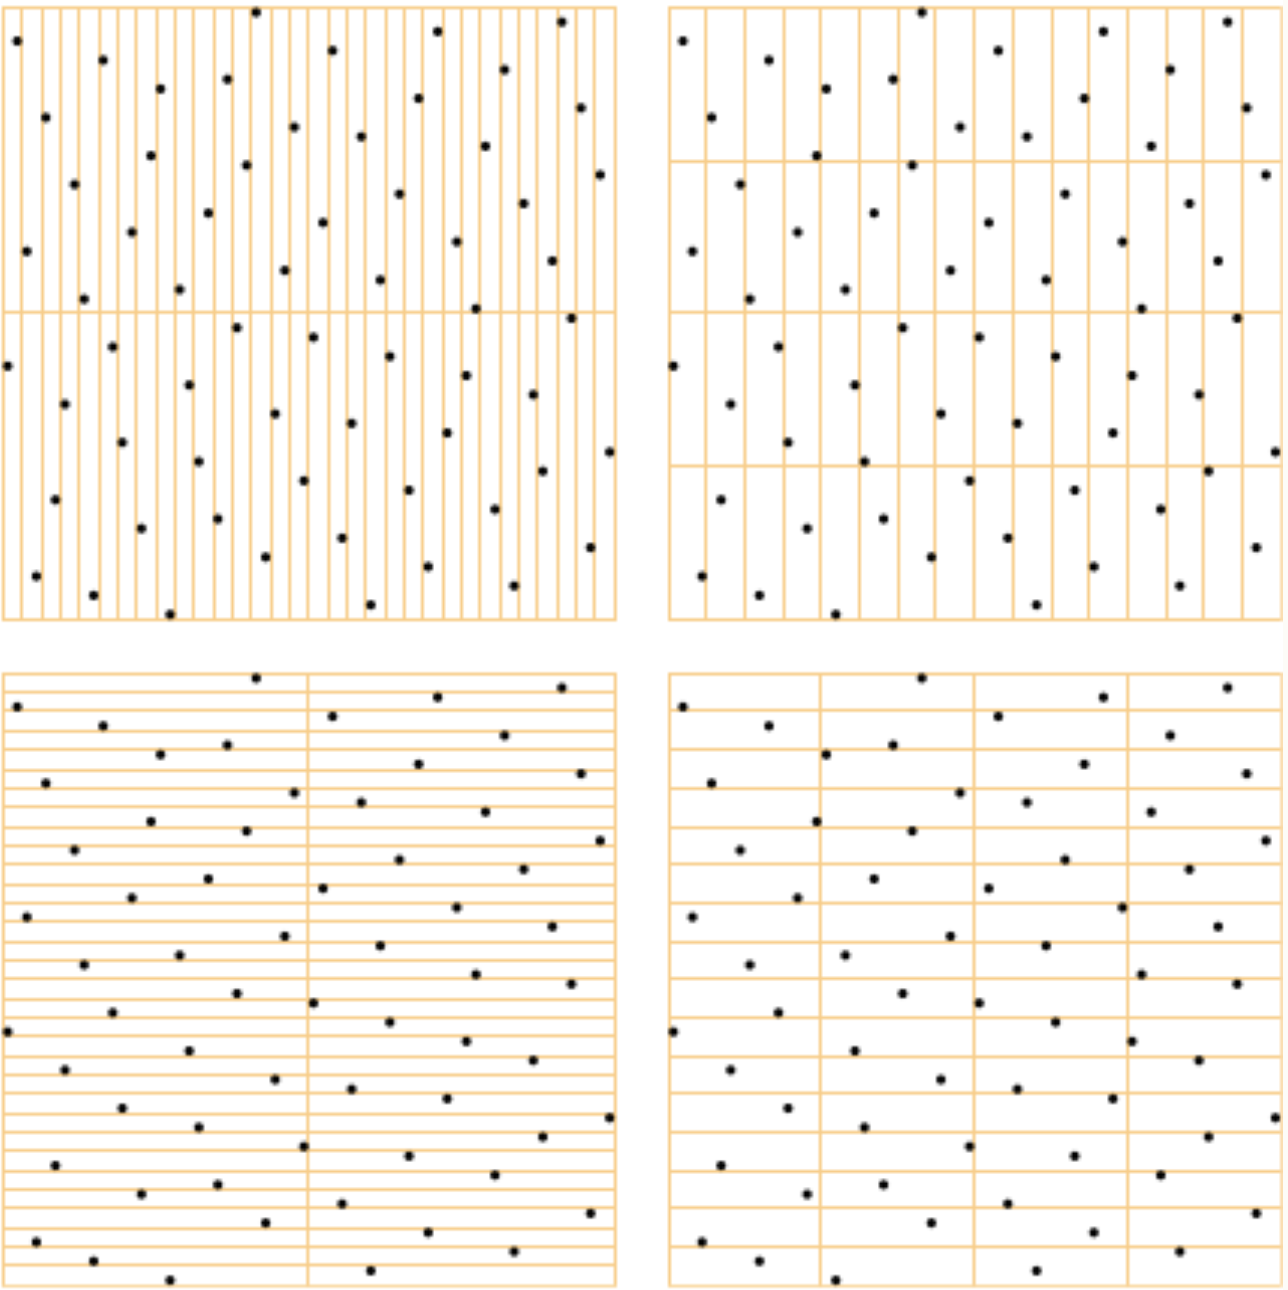
\includegraphics[width=110mm]{target/diadic_nets.png}\\
        This figure from \cite{dyadic} illustrates this concept well
    \end{figure}    
    
    \> \textit{Intuition}. The intuition is that a low discrepancy sampler is by definition
        really good in integrate axis-align rectangle. Thus, for every rectangle inside a 
        subspace, the point set needs to be good. And we want to apply the same idea with
        our 3D generalisation. We want that for each sub 3D rectangle of the cube, if we
        take only the point inside this sub rectangle, we still have good 2D projection.  

\subsubsection{Application in 2D}

    \> To better understand what I am talking about with multiclass sampling, let's look at
    low discrepancy sampler. The definition of the discrepancy is:
    \[ D_N^*(B,s) = \sup_{b\in B} \left | \frac{card(x_k \in b)}{N} - Vol(b)\right |\]
    where $B = \{[v_1,v_2]\times[v_3,v_4] | v_1,v_2,v_3,v_4 \in [0,1]\}$ is the set of all 
    rectangle inside the unit square and $Vol(b)$ the volume of the rectangle $b$. We can then write $B$ as 
    \[B =  \bigcup_{v_1,v_2} B_{v_2}^{v_1} = 
    \bigcup_{v_1,v_2} \{[v_1,v_2]\times[v_3,v_4] | v_3,v_4 \in [0,1]\}\]

    \> We can't directly optimize for the discrepancy due to the $\sup$, but we can optimize
    for all the terms inside the $\sup$.

    \> \textit{Observation}. If we set $v_1$ and $v_2$, and take only the points where the
    X-coordinate is between $v_1$ and $v_2$. And then optimize those point such that their 
    Y-coordinate form a blue noise. It is equivalent to optimise for:
    \[ \sup_{b\in B_{v_2}^{v_1}} \left | \frac{card(x_k \in b)}{N} - Vol(b)\right | \]

    \> With this in mind, we can optimize our sample to get different result.
    We don't necessarily have to optimize for all size of sub rectangle. If we choose
    some well chosen fixed size, we can produce sample close to classical algorithm. 
    In the table below, there is different sample produce by choosing well the size off
    rectangle we want to optimize for.

    \begin{figure}[H]
        \centering
        \begin{tabular}{|C{5cm}|C{2.5cm}||C{3cm}|L{3cm}|}
        \hline parameter & equivalent & points & spectrum \\
        \hline  
            $\{\sqrt N\}$ & 
            regular grid &
            \frame{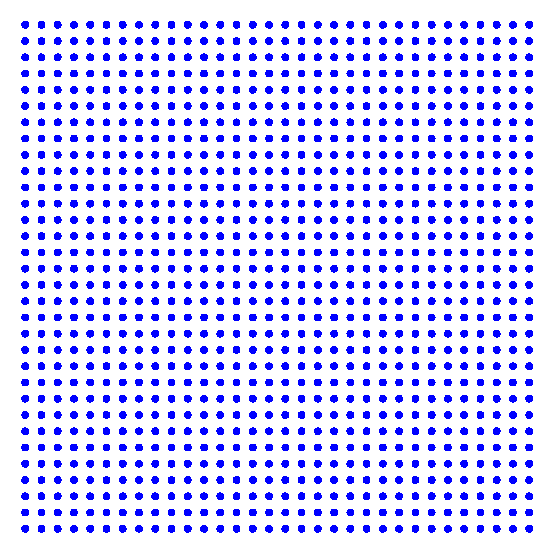
\includegraphics[width=30mm]{sample/ours_grid.pdf}} & 
            \frame{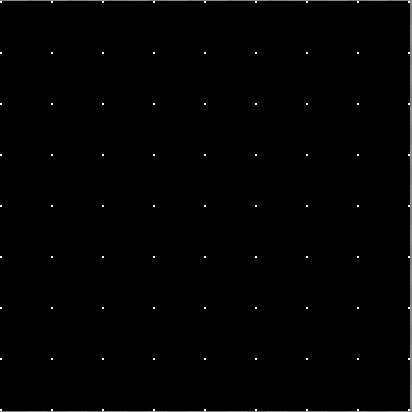
\includegraphics[width=30mm]{sample/ours_grid_spectrum.png}} 
            % $0.0310058593750000$  \\
        \tabularnewline
        \hline  
            $\{1,\sqrt N\}$ toroïdale& 
            correlated multi jitter &
            \frame{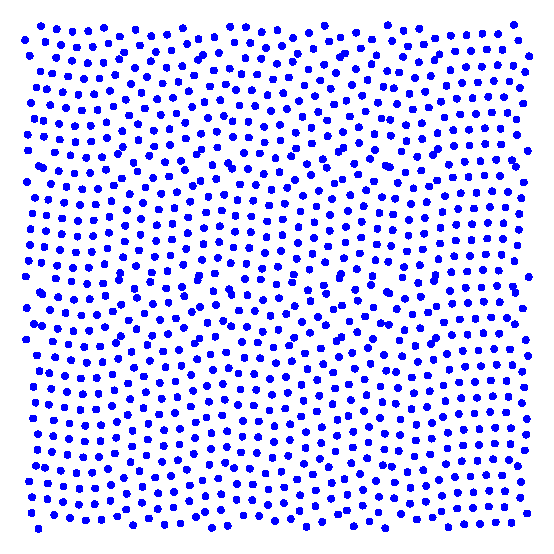
\includegraphics[width=30mm]{sample/ours_cmj.pdf}} & 
            \frame{\includegraphics[width=30mm]{sample/ours_cmj_spectrum.png}}
            %$0.0067580312558710$  \\
        \tabularnewline
        \hline  
            $\{2^i | i < \log_2(N) \}$ toroïdale & 
            dyadic nets &
            \frame{\includegraphics[width=30mm]{sample/ours_dyadic.pdf}} & 
            \frame{\includegraphics[width=30mm]{sample/ours_dyadic_spectrum.png}} 
            %$0.0067580312558710$  \\
        \tabularnewline
        \hline 
            $\{i | i < \sqrt N \}$ toroïdale & 
            no real equivalent &
            \frame{\includegraphics[width=30mm]{sample/ours_low.pdf}} & 
            \frame{\includegraphics[width=30mm]{sample/ours_low_spectrum.png}} 
            %$0.0067580312558710$  \\
    \tabularnewline
    \hline 
        \end{tabular}\\

        \textit{The parameter is the set of the inverse of the size of rectangle
        we optimized for.}
    \end{figure}
    
    \> As the plot show, we can get some nice sample. Even if we only optimized
    axes-align direction. The way we optimized axis align is describe in the 
    Annexe A.2. It is just optimization for a Blue Noise in 1D.

\subsubsection{Application in 3D}
    With the same idea than before, we can try to make our naive 3D generalisation attempt
    better, by making some multi-class sampling. But I didn't have enough time to produce
    something satisfying.


\subsection{Other metric}

Let's go back to our modified SOT:
\[SW_p(\mu, \nu) = \int_{\mathbb{S}^{d-1}} \gamma(\theta) W_p(\mu^\theta,\nu^\theta) d\theta\]
I wanted to understand why it works. I then noticed that we can rewrite this equation by merging
the distance with $\gamma$. 
\begin{align*}
    SW_p(\mu, \nu) &= \int_{\mathbb{S}^{d-1}} \gamma(\theta) W_p(\mu^\theta,\nu^\theta) d\theta \\
    &= \int_{\mathbb{S}^{d-1}} \left (\inf_{\pi \in \Gamma{\mu,\nu}} \int_{\mathcal X^2} 
    (\gamma(\theta) \lVert x-y \rVert)^p d\pi(x,y) \right )^{1/p} d\theta \\
    &= \int_{\mathbb{S}^{d-1}} \left (\inf_{\pi \in \Gamma{\mu,\nu}} \int_{\mathcal X^2} 
    \tilde d(x,y) d\pi(x,y) \right )^{1/p} d\theta \\
    &= \int_{\mathbb{S}^{d-1}} \tilde W_p(\mu^\theta,\nu^\theta) d\theta
\end{align*}
By doing so, it is like doing Slice Optimal Transport but with a
new metric.

\> Generally, in most of the method, people usually use the $L_2$ distance. But why don't we
try other metric? Maybe we could get different and better result. Thus, we will change
the metric in three classical method by those one:
    \begin{itemize}
        \item $L_2$ distance: $d(a,b) = (b.x-a.x)^2 + (b.y-a.y)^2$
        \item $L_\infty$ distance: $d(a,b) = \max( |b.x-a.x|, |b.y-a.y|)$
        \item $L_2$ twisted: $d(a,b) = 4(b.x-a.x)^2 + (b.y-a.y)^2$ with a rotation of $\pi/6$.
        \item cross distance: $d(a,b) = max(dmin,dmax/10)$ \\
            where $dmin = \min(|b.x-a.x|, |b.y-a.y|)$ and $dmax = \max(|b.x-a.x|, |b.y-a.y|)$.
    \end{itemize}
\> \textit{Remark}. The last one isn't even really a semi-metric. It's a semi-metric, 
    that means that the triangular inequality is no longer true with it. But at least,
    it is linear center in 0. ($d(\lambda x,0) = \lambda d(x,0)$).

\subsubsection{Dart-throwing algorithm}
    The easiest way to test different metric is to do some dart throwing, but with weird
    shape for reject new sample.

    \begin{figure}[H]
        \centering
        \begin{tabular}{cccc}
        \frame{\includegraphics[width=33mm]{sample/dart_blue.pdf}}
        & \frame{\includegraphics[width=33mm]{sample/dart_square.pdf}}
        & \frame{\includegraphics[width=33mm]{sample/dart_twisted.pdf}}
        & \frame{\includegraphics[width=33mm]{sample/dart_cross.pdf}}
        \\[3pt]
        \frame{\includegraphics[width=33mm]{sample/dart_blue_spectrum.png}}
        & \frame{\includegraphics[width=33mm]{sample/dart_square_spectrum.png}}
        & \frame{\includegraphics[width=33mm]{sample/dart_twisted_spectrum.png}}
        & \frame{\includegraphics[width=33mm]{sample/dart_cross_spectrum.png}}
        \\[3pt]
        \textit{$L_2$ distance} 
        & \textit{$L_\infty$ distance} 
        & \textit{$L_2$ twisted} 
        & \textit{cross distance}
        \end{tabular}
    \end{figure}

\> \textit{Discussion}. This method clearly show the metric we used. But unfortunately, 
it only produce low quality blue noise.

\subsubsection{Wasserstein Method}
    But Wasserstein method could be also adapted to change the metric. Since the algorithm
    doesn't depend on the metric used.
    \begin{figure}[H]
        \centering
        \begin{tabular}{cccc}
        \frame{\includegraphics[width=33mm]{sample/WBN_blue.pdf}}
        & \frame{\includegraphics[width=33mm]{sample/wbn_square.pdf}}
        & \frame{\includegraphics[width=33mm]{sample/wbn_twisted.pdf}}
        & \frame{\includegraphics[width=33mm]{sample/wbn_cross.pdf}}
        \\[3pt]
        \frame{\includegraphics[width=33mm]{sample/WBN_blue_spectrum.png}}
        & \frame{\includegraphics[width=33mm]{sample/wbn_square_spectrum.png}}
        & \frame{\includegraphics[width=33mm]{sample/wbn_twisted_spectrum.png}}
        & \frame{\includegraphics[width=33mm]{sample/wbn_cross_spectrum.png}}
        \\[3pt]
        \textit{$L_2$ distance} 
        & \textit{$L_\infty$ distance} 
        & \textit{$L_2$ twisted} 
        & \textit{cross distance}
        \end{tabular}
\end{figure}
    \> \textit{Remark}. The cross distance doesn't work at all for this method. An explanation
    is that in this method, we approximate the uniform density with a grid. Thus, our sample
    with this metric tends to be align on this grid. A naive solution could be to make this grid more dense, but it will be to big to compute.
    
\subsubsection{Relaxation Method}
    One simple way to create blue noise is to simulate a physic system where each points
    repel each other. With this method, it is also easy to chose a different metric.
    \begin{figure}[H]
        \centering
        \begin{tabular}{cccc}
        \frame{\includegraphics[width=33mm]{sample/rbn_blue.pdf}}
        & \frame{\includegraphics[width=33mm]{sample/rbn_square.pdf}}
        & \frame{\includegraphics[width=33mm]{sample/rbn_twisted.pdf}}
        & \frame{\includegraphics[width=33mm]{sample/rbn_cross.pdf}}
        \\[3pt]
        \frame{\includegraphics[width=33mm]{sample/rbn_blue_spectrum.png}}
        & \frame{\includegraphics[width=33mm]{sample/rbn_square_spectrum.png}}
        & \frame{\includegraphics[width=33mm]{sample/rbn_twisted_spectrum.png}}
        & \frame{\includegraphics[width=33mm]{sample/rbn_cross_spectrum.png}}
        \\[3pt]
        \textit{$L_2$ distance} 
        & \textit{$L_\infty$ distance} 
        & \textit{$L_2$ twisted} 
        & \textit{cross distance}
        \end{tabular}
\end{figure}


\subsubsection{Discussion}
    \> This idea of changing the metric doesn't really work well. As the result shows, if
    we have a semi-metric (the cross), most of the method aren't adapted. Moreover, as 
    explained in
    [\cite{singh17convergence}], even if we get the shape we desire in the power spectrum,
    it won't improve the overall convergence rate. 
    But, at least, it seems that the shape of the metrcic used appear in the power spectrum.

    \> Unfortunately, I didn't manage to formally proove this conjecture: 
    \textit{The shape of the power spectrum is the shape of the metric used}.
    At best, we can get some intuition thanks to the strong link between the power
    spectrum and the PCF.

\section{To go further}

\subsection{A better 3D generalization}
    \> The next thing to test that I didn't have the time to do is to optimize directly 
    in the 3D space. And we should be able to have some clear improvement over our attempt
    to 3D generalization, even upgraded with multi-class sampling.

\subsection{Multi-layer Perceptron}
    One issue we have with all this optimization method, is that it take so much times
    to generate any sample. But since all our method are base on optimization, it is
    "easy" to train an MLP that can produce the same result. It will be very to
    optimize it, but once it's done, it will allow use to produce sample really fast,
    in real time.\\

\section{Conclusion}
    \> During this internship I touched well more things than I initially expected.
    The objetive before starting was to create samples for motion blur and depth of field
    that are better than low discrepancy sampler, using slice optimal transport.

    \> I didn't managed to fullify this objective, but I explored others things:
    \begin{itemize}
        \item I started by exploring the link between sample and their power spectrum
            with the radial average method.
        \item I then used the Slice Optimal Transport method, and produce samples
            with anisotropic power spectrum. But I had to be bit smarter to convert those
            anisotropic power spectrum into an improvement of the integration convergence 
            rate.
        \item But then I tried to make a naive 3D generalisation, and tried to apply this for
            real scene wit motion blur. But it didn't work at all.
        \item
            I then realize that our 3D generalization wasn't the good idea, and that we may 
            be able to improve with multiclass sampling. Thus, I explore a way of doing
            multi class sampling in 2D to better understand it.
        \item In parallel, I wanted to understand why this method based on Slice Optimal
            Transport work. And so, I explore the idea of changing the metric used to compute
            the distance between point.
    \end{itemize}
    There are still many thing thing to explore and to prove, like other 3D generalisation
    or explore deeper multiclass sampling and the changing metric idea. Moreover, how to
    reduce the time used to optimized with some machine learning.
    

\printbibliography[title={Bibliography}] % Print the bibliography, section title in curly brackets

\newpage

\appendix

\section{Optimal Transport}

\subsection{Optimal transport definition}

\> \textit{Wasserstein distance}. The optimal transport distance between two 
    probabilistic measures with $L_p$ norm is:
    \[W_p(\mu, \nu) = \left (\inf_{\pi \in \Gamma{\mu,\nu}} \int_{\mathcal X^2} 
                    \lVert x-y \rVert^p d\pi(x,y) \right )^{1/p}\]
    where $\Gamma(\mu,\nu)$ is the set of all continue transformation from 
    $\mu$ to $\nu$.

\> \textit{Slice Wasserstein distance}. The slice optimal transport distance 
    between two probabilistic measures with $L_p$ norm is:
    \[SW_p(\mu, \nu) = \int_{\mathbb{S}^{d-1}} W_p(\mu^\theta,\nu^\theta) d\theta\]
    where $\theta \in \mathbb{S}^{d-1}$ is a point on the $(d-1)$-dimensional sphere, 
    and $\mu^\theta$ and $\nu^\theta$ are the Radon transforms (i.e., orthogonal 
    projections) of the measures onto the line through $\theta$.


\> \textit{Blue Noise with Wasserstein distance}. In this work we are 
    interested in approximating uniform probabilistic measures $\nu$ by a 
    point set $X = \{x_i\}_{i=1}^n$ on some Euclidean domain $\mathcal X$. 
    The quality of this approximation can be quantified by the Wasserstein 
    distance $W(X, \nu)$. 
    And the result of doing so, make $X$ to follow a blue noise distribution.

\subsection{1D Optimal Transport}
\noindent In the case of $p=1$, we have :
\begin{align*}
    W_1(X,\mu) &= \int_0^1 |F_X^{-1}(x) - F_\mu^{-1}(x)| dx \\
               &= \sum_{i=1}^N \int_{\frac{i}{N}}^{\frac{i+1}{N}} |x_i - F_\mu^{-1}(x)| dx
\end{align*}
Thus, we want to find the $X$ that minimize this distance. For each $x_i$, we want to minimized
\[ \int_{\frac{i}{N}}^{\frac{i+1}{N}} |x_i - F_\mu^{-1}(x)| dx \]
The minimum is achieve in the median, in other word $x_i = F_\mu^{-1}\left (\frac{i+0.5}{N} \right )$


\section{Blue noise optimization methods}

\subsection{Blue noise with radial average target}

\subsubsection{Compute Radial Average Power Spectrum}
Formally, the radial average power spectrum (normalized) in $\rho$ is:
\begin{align*}
    radial(\rho) & = \frac{N}{V(\rho)}\int_{\mathbb{S}^{d-1}} \mathcal P_S(\rho \textbf{n}) d\textbf{n} \\
        &= \frac{1}{V(\rho)} \int_{\mathbb{S}^{d-1}} \frac{1}{N}\left \Vert \sum_{j=0}^N e^{-2i\pi(\rho \textbf{n}\cdot x_j)}  \right \Vert^2 d\textbf{n} \\
        &= \frac{1}{V(\rho)} \int_{\mathbb{S}^{d-1}} \frac{1}{N} \left [ \left ( \sum_{j=0}^N \cos(2\pi\rho \textbf{n}\cdot x_j) \right )^2 + \left ( \sum_{j=0}^N \sin(2\pi\rho \textbf{n}\cdot x_j) \right )^2\right ]  d\textbf{n}
\end{align*}  
Since, we can't compute there integral, we approximate it by making a Monte Carlo integration. ($P$ is a finite subset of $\rho\mathbb{S}^{d-1}$).
    \[ radial(\rho) \approx \frac{1}{|P|} \sum_{p\in P} \frac{1}{N} \left [ \left ( \sum_{j=0}^N \cos(2\pi p\cdot x_j) \right )^2 + \left ( \sum_{j=0}^N \sin(2\pi p\cdot x_j) \right )^2\right ] \]

\subsubsection{What we want to do:}
We cant to target a specific radial average spectrum $target$. To do so, we do a gradient descent.
Formally, is we want to minimize:
\[ E = \int_0^\infty (target(\rho) - radial(\rho))^2 d\rho \]
\> \textit{Remark}. But, in reality, we don't really car about the radial average for high $\rho$ value. So we want to minimized only :
\[ E = \int_0^a (target(\rho) - radial(\rho))^2 d\rho \]
where $a$ is about $O(N^{1/d})$.

\subsubsection{Derivative of Radial Average Power Spectrum}
In order to minimize, we need to compute the derivative of $E$ according to every $x_i$. 
\begin{align*}
    \frac{\partial E}{\partial x_i} &= \frac{\int_0^a (target(\rho) - radial(\rho))^2 d\rho}{\partial x_i} \\
    &= \int_0^a \frac{\partial \left [(target(\rho) - radial(\rho))^2\right ]}{\partial x_i}d\rho \\
\end{align*}
Since, $E$ is a sum of value, to simplify the following computation, we just need to compute:
\begin{align*}
    \frac{\partial \left[ (target(\rho) - radial(\rho))^2\right ]}{\partial x_i} 
        &= -2((target(\rho) - radial(\rho))\frac{\partial radial(\rho)}{\partial x_i}
\end{align*}
Where :
\begin{align*}
    \frac{\partial radial(\rho)}{\partial x_i} = \frac{1}{|P|} \sum_{p\in P} \frac{1}{N} & \left ( -4\pi p \sin(2\pi p\cdot x_i) \sum_{j=0}^N \cos(2\pi p\cdot x_j) \right )\\
    &\qquad+ \left ( 4\pi p \cos(2\pi p\cdot x_i) \sum_{j=0}^N \sin(2\pi p\cdot x_j) \right)
\end{align*}

\subsubsection{Implementation}
With those formulation, by making sure to not do twice the same computation, we can
compute the derivative of $E$ in $O(N|P|)$. And then, we can make the classical gradient
descent algorithm on top of it.

\subsection{Blue noise by relaxation}

We just simulate a physic system where each point repel each other. The coefficent of the
repultion between $x_i$ and $x_j$ is:
\[c_{ij} = \exp(-2N\times d(x_i,x_j)^2) \]
where $d(x_i,x_j)$ is the distance between $x_i$ and $x_j$.

\subsection{Optimal Transport Blue Noise}

\subsubsection{General idea}

If we take $\nu$ a discrete probabilistic measures $X = (x_i)_i$, and $\mu$ a uniform probabilistic measures.
The result of optimizing the Wasserstein distance along $\nu$ make $\nu$ follow a Blue Noise 
distribution. 

We use the the same algorithm and idea described in [\cite{BlueNoiseWassertein}]. 

Here a quite description of the algorithm.
The algorithm has 3 step:
\begin{itemize}
    \item we compute the distance matrix between the two distribution.
    \item we compute the optimal transport distribution $\Pi$ with this distance.
    \item we compute the optimal $\mu$ according to this optimal distribution $\Pi$.
\end{itemize}
We repeat those three step until we have converge.

\begin{algorithm}
    \caption{Wasserstein Blue Noise}
    \label{euclid}
    \begin{algorithmic}[1] % The number tells where the line numbering should start
        \Procedure{Main}{$a,b$}
            \State $X \gets$ RandomDistribution()
            \While{X has not converged}
                \State $D \gets$ UpdateDistance()
                \State $\Pi \gets$ BregmanProjections()
                \State $OptimalX \gets $ OptimalX()
                \State $X \gets lerp(X,OptimalX,theta)$ \Comment{We do a lerp to control the size of each step}
            \EndWhile\label{euclidendwhile}
            \State \textbf{return} $X$\Comment{The optimal distribution is X}
        \EndProcedure
    \end{algorithmic}
\end{algorithm}

\subsubsection{Proof of the algorithm}

The first step is straight forward, but it's important because it allow us to use 
some unusual metric distance.

To do the second step,we use Bregman Projection [\cite{BregmanProjection}]. The algorithm
is describe in the paper of Benamou.

The last step, is just a minimization of the energy function parameterize by $\mu$ :
\[ E(\mu) = W_p(\mu, \nu) = arg \min_{\Pi} <D,\Pi> - \epsilon H(\Pi) \]
Since we fixed $\Pi$, we have:
\begin{align*}
    \frac{\partial E}{\partial \mu} &= \frac{\partial <D,\Pi>}{\partial \mu} \\
\end{align*}
In the case of $d(x,y)$ is the $L_2$ norm. We can easily compute the minimum of this function 
because the function $E$ is convex. If $\frac{\partial E}{\partial \mu} = 0$, then we have
\begin{align*}
    0 &= \frac{\partial E}{\partial x_i}\\
    0 &= \sum_{(x,y)\in X\times Y} \rho_i \frac{\partial d(x,y)}{\partial xi}\pi(x,y) \\
    0 &= \sum_{(y)\in Y} 2(x_i - y)\pi(x,y) \\
    x_i &= \sum_{y \in Y} y \pi(x,y) \rho_i^{-1}
\end{align*}
Thus, we can summarize that by : $X = Y \Pi^T diag(\rho^{-1})$
But more generally, if we have another metric, we can compute the minimum by simply doing a 
gradient descent on the energy function.

\subsection{Slice Optimal Transport Blue Noise }
    
\subsubsection{Theory}
    We use the same thing that [Paulin 2020] did.

    \> To do so, we need to be able to compute the orthogonal projection integral $F$
    of a uniform density. We need the inverse $F{-1}$ of this function. And we want to 
    compute
    $F^{-1}(x)$ for all $x \in \{\frac{i+0.5}{N}, i \in \llbracket 1,N \rrbracket\}\: 
        \widehat = \:\mathcal I$.
    The way we compute those is describe later. The proof of this is in annex A
    

    \> We added something to their method, corresponding to what Corentin did. In order to 
    homogenized the gradient everywhere on the square, we had a normalization term to the 
    gradient that correspond to the value of the projective density around or point.


%\subsubsection{Density of a circle projected {\color{red} TO DO : add a schema}} 
%    One remark is that the projected density is the same for every $\theta \in 
%    \mathbb{S}^{d-1}$.
%    The function that describe a semi-circle is $f(x)^2 + x^2 = 1$. Thus
%    it is $f(x) = \sqrt{1-x^2}$, for $x \in [-1,1]$. We want to compute:
%    \begin{align*}
%        F(x) &= \frac{2}{\pi}\int_{-1}^{x} \sqrt{1-t^2} dt \\
%             &= \frac{1}{\pi}\left (x\sqrt{1-x^2} + \sin^{-1}(x) + \frac{\pi}{2}\right )
%    \end{align*}
%    As we want $F^{-1}(x)$ and this function is to complex, we approximate $F^{-1}(x)$
%    by making a dichotomy on $F$. (We can do it because $F$ is increasing). We can do item
%    only one time in pre-computation as this projection doesn't depends on $\theta$. 

\subsubsection{Density of a square projected}
    \begin{figure}[H]
        \centering
        \includegraphics[width=110mm]{schema/schema_square.png}\\
    \end{figure}   

    Let $x_0,x_1,x_2$ and $x_3$ be ordered projected value of the vertex of the square.
    \begin{itemize}
        \item $x < x_0$, we have $F(x) = 0$
        \item $x \in [x_0,x_1]$, we have  $F(x) = (x-x_0)^2a$
        \item $x \in ]x_1,x_2]$, we have  $F(x) = (x-x_1)d + F(x_1)$
        \item $x \in ]x_2,x_3]$, we have  $F(x) = 1 - (x_3-x)^2a$
        \item $x > x_3$, we have $F(x) = 1$
    \end{itemize}
    with $a =  \frac{1}{2(x2-x0)(x1-x0)}$ and $d = \frac{1}{2}\sqrt{1 + (x1-x0)^2/(x2-x0)^2}$ \\
    Thus, we can directly compute the density inverse:
    \begin{itemize}
        \item For $x \in [0,F(x_1)]$, we have $F^{-1}(x) = \sqrt{x/a} + x_0$.
        \item For $x \in [F(x_1),F(x_2)]$, we have $F^{-1}(x) = (x-y1)/d + x_1$.
        \item For $x \in [F(x_2),1]$, we have $F^{-1}(x) = x3 - \sqrt{(1-x)/a}$.
    \end{itemize}
    
\> \textit{Remark}. There is on degenerate case, when $x_0=x_1$. But this case can easily 
    be manage because it correspond to a projection on one of the vector of the orthogonal
    basis. Thus, in this case, $F(x) = x$, so it is even easier.
    
\> \textit{Complexity analysis}. This is not really expensive to compute, it is only $O(1)$     for each evaluation. Thus, we will compute this each time we need it.

\end{document}